\documentclass{article}
\usepackage[utf8]{inputenc}
\usepackage{amsmath}
\usepackage{amssymb}
\usepackage{minted}
\usepackage{tikz}
\usetikzlibrary{positioning}
\usepackage[ruled,vlined]{algorithm2e}

\title{COMS 527 Proposal}
\author{Justin Stanley}
\date{October 15, 2021}

\begin{document}

\maketitle

\section{Summary}

For the class project I would like to train a neural network to play the game Connect 4. The model training will be distributed across multiple computers using multithreading and MPI. Nodes with GPUs will use CUDA to accelerate model performance. The model will train with reinforcement learning only through self-play, without access to any human training data. A terminal game position is illustrated on page \pageref{fig:c4}.

\begin{figure}
    \centering
    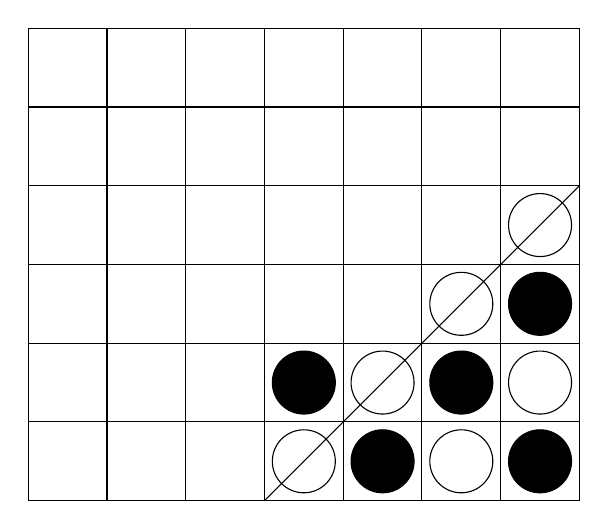
\begin{tikzpicture}
        \draw (0,0) -- (7,0);
        \draw (0,1) -- (7,1);
        \draw (0,2) -- (7,2);
        \draw (0,3) -- (7,3);
        \draw (0,4) -- (7,4);
        \draw (0,5) -- (7,5);
        \draw (0,6) -- (7,6);
        \draw (0,0) -- (0,6);
        \draw (1,0) -- (1,6);
        \draw (2,0) -- (2,6);
        \draw (3,0) -- (3,6);
        \draw (4,0) -- (4,6);
        \draw (5,0) -- (5,6);
        \draw (6,0) -- (6,6);
        \draw (7,0) -- (7,6);
        \draw (3.5, 0.5) circle (0.4);
        \filldraw (4.5, 0.5) circle (0.4);
        \filldraw (3.5, 1.5) circle (0.4);
        \draw (4.5, 1.5) circle (0.4);
        \draw (5.5, 0.5) circle (0.4);
        \draw (6.5, 3.5) circle (0.4);
        \draw (5.5, 2.5) circle (0.4);
        \filldraw (6.5, 2.5) circle (0.4);
        \filldraw (5.5, 1.5) circle (0.4);
        \filldraw (6.5, 0.5) circle (0.4);
        \draw (6.5, 1.5) circle (0.4);
        \draw (3,0) -- (7, 4);
        
    \end{tikzpicture}
    \caption{Connect-4 game, winning state for white}
    \label{fig:c4}
\end{figure}

\vspace{0.5cm}

\noindent\textbf{Goals}
\begin{itemize}
    \item Final model should consistently win against random moves
    \item Model training/inference speed should scale with GPU count across nodes
    \item Model skill progression should be measurable
\end{itemize}

\vspace{0.5cm}

\noindent\textbf{Limitations}
\begin{itemize}
    \item Each node must have at least one GPU to contribute
\end{itemize}

\section{Implementation}

\subsection{Libraries}

The project will be written in C++, using MPI for concurrency with distributed memory. Torch will be used for neural network training and inference. The source code will be documented using Doxygen.

\subsection{Architecture}

The agent will use a directed Monte-Carlo tree search to make decisions. The search will be led by policy and value outputs from the neural network. Training data will be built in parallel across all nodes, however once the training data is ready the training step can take place on a single node.
Each node will have access to an archive of past games played. Every GPU will play 32 games simultaneously to contribute to the experience buffer.

\subsection{Evaluation}

The agent will be evaluated by playing $n$ games against a random policy network (effectively plain MCTS). Let a loss count as 0 points, a draw count as $\tfrac{1}{2}$ points, and a win count as 1 point. We let $s$ be the total score after $n$ games. The model performance function is then
$$p(s, n) = \dfrac{s}{n}.$$
The initial model is expected to have a performance rating close to 0.5, but as the model progresses the performance rating should tend towards 1. Performance evaluations will be run every 25 iterations of the network.

\end{document}
